%% Documentclass:
%% Network Neuroscience
\documentclass[NETN,manuscript]{stjour-new}

%%%%%%%%%%% Article Set-Up %%%%%%%%%%%%%%%%%%%%%%%%%%%%%%%%%%%%
%% Article Type:
%% Default is Research.

%% Or, choose one of these options:
%% Research, Methods, Data, Review, and Perspective

\articletype{Perspective}

%%%%%%%%%%%%%%%%%%%%%%%%%%%%%%%%%%%%%%%%%%%%%%%%%%%%%%%%%%%%%%%
%% author definitions should be placed here:

%% example definition
\def\taupav{\tau_{\mathrm{Pav}}}

%% common path to your figure files (for organization purposes)
\graphicspath{{figs/}}

\begin{document}
\title[Who You Gonna Believe?]{Who You Gonna Believe, Me or Your Lying Eyes}
\subtitle{Fake News Early Detection Using Graph Neural Networks}

%% If shortened title for running head is needed so that the article title can fit
%%   in the running head, use [] argument, ie,
%%
%%   \title[Shortened Title for Running Head]{Title of Article}
%%   \subtitle{Subtitle Here}

%% Since we use \affil{} in the argument of the \author command, we
%% need to supply another version of the author names, without \affil{}
%% to be used for running heads:

\author[John Hawthorne Smith]
{John Hawthorne Smith\affil{1}}

\affiliation{1}{Masters of Science in Data Science, Northwestern University, Evanston, United States}

%ie.
%\affiliation{1}{Gatsby Computational Neuroscience Unit, University
%College London, London, United Kingdom} 


\correspondingauthor{John Hawthorne Smith}{JohnSmith2020@u.northwestern.edu}

% ie,
%\correspondingauthor{Ritwik K. Niyogi}{ritwik.niyogi@gatsby.ucl.ac.uk}

\keywords{(a series of capitalized words, separated with commas)}

%ie
%\keywords{Work, Leisure, Normative, Microscopic,  Reinforcement Learning, Economics}

\begin{abstract}
Abstract text here.
\end{abstract}



\section{Introduction}
In 2018, social media overtook print media as the fourth most popular source of news for Americans. As of 2019, 20 percent "often" got their news from social media \citep{shearer2018social}, while 68 percent of all American gets their news from social media at least occasionally \citep{matsa2018news}. This is not inherently a bad thing - in countries with authoritarian leaders and state-run media, social media may be the only outlet for opposition spokespeople to share their messages \citep{walker2014breaking}; ordinary citizens can now contribute their stories and experiences without the high financial barrier to entry that traditional journalism requires \citep{qualman2012socialnomics, tapscott2008wikinomics}; in unmanageable situations and crises, such as the 2017 Manchester bombing, social media allowed for the instantaneous exchange of information between individuals and emergency management agencies \citep{mirbabaie2020breaking, eriksson2016facebook}; in situations like the COVID-19 pandemic, where information is rapidly evolving, social media allows for immediate knowledge dissemination by dramatically shortening the traditional time from publication to widespread translation to adoption \citep{chan2020social}. Furthermore, experts can readily reach followers who may not have deep knowledge of a subject - Dr. Esther Choo has over 113,000 followers – and can increase awareness of public health needs and crises, while openly debating other experts and answering direct questions \citep{gottlieb2020information}.

However, not all information shared on social media is true, and the subset of people who primarily get their news from social media tend to be less engaged, less knowledgeable of current events, more likely to hear unproven claims and conspiracy theories than those who get their news from more traditional sources, and are more likely to believe these conspiracies \citep{mitchell2020americans}. In December 2016, Edgar Maddison Welch drove from North Carolina to Washington D.C. with an AR-15 to investigate a fake pedophile conspiracy ring known as "pizzagate" \citep{goldman2016comet}. In 2018, Burmese officials created over 1,000 Facebook posts filled with hate speech and detailing fake crimes committed by the Rohynga Muslim minority to justify one of the largest forced migrations in recent history \citep{subedar2018country}.

Exacerbating this problem, the spread of correct information does not always travel as quickly or reach as broad of an audience as misinformation does \citep{maddock2015characterizing, vosoughi2018spread}, and, in some cases, rumors and other fake stories actually see an increase in spread \textbf{after} they have been debunked \citep{starbird2014rumors}. In the case of the "pizzagate" conspiracy, several news outlets -- including the Washington Post, New York Times, and Snopes -- had debunked the story several months before Welch decided to drive to Washington D.C. \citep{kang2016fake,lacapria2016fact,board_2016}, yet pro-conspiracy posts on Facebook, Instagram, YouTube, and Twitter actually saw a sharp uptick as the supporters became more zealous \citep{kang2016washington}. In fact, this fits a pattern where highly controversial and politicized topics spark backfire effects when passionately held misconceptions are challenged \citep{gollust2009polarizing,nyhan2010corrections,nyhan2013hazards,redlawsk2010affective,schaffner2016misinformation}.


 \begin{figure}[htp]
    \centering
    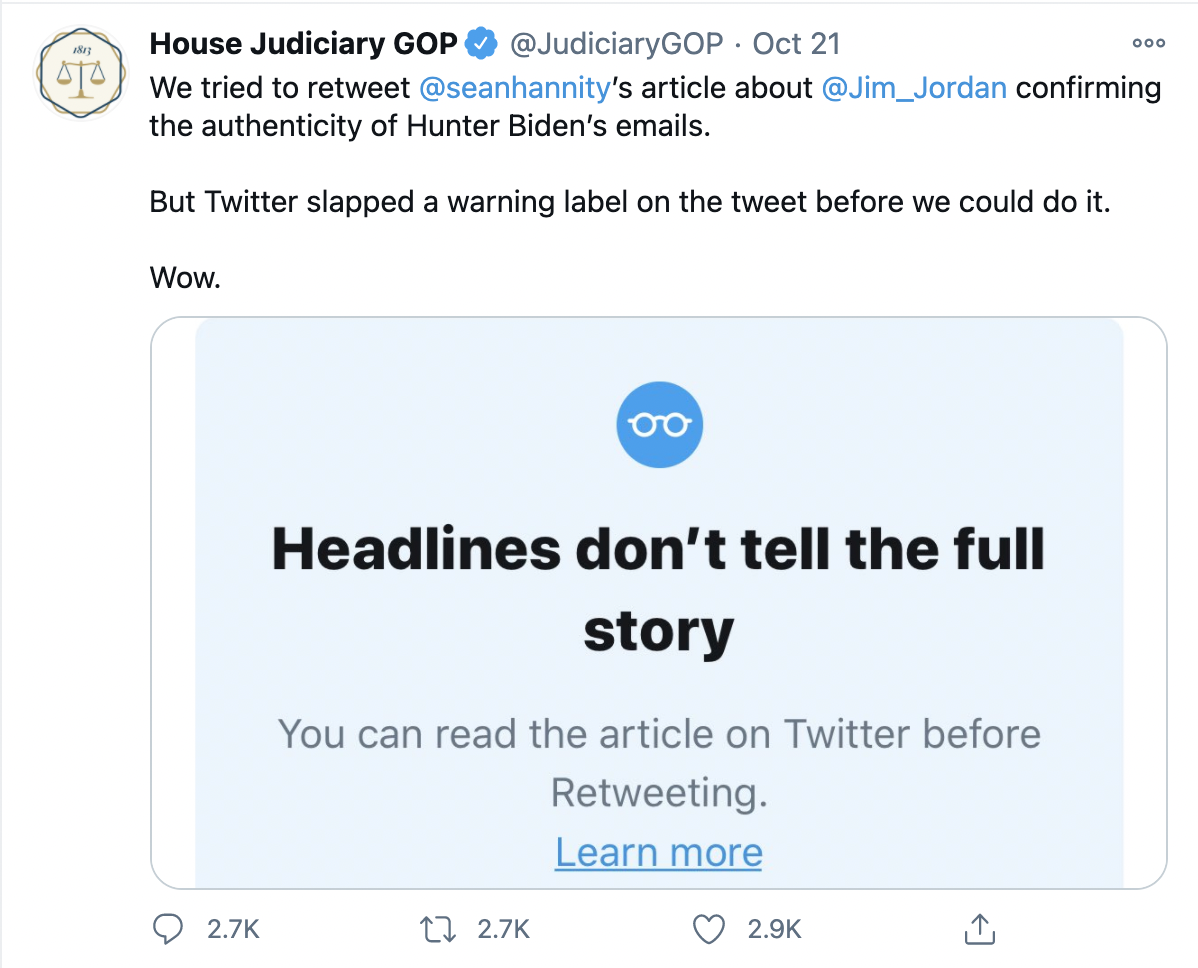
\includegraphics[width=4cm]{JudiciaryTweet.png}
    \caption{JudiciaryTweet}
    \label{img:JudiciaryTweet}
\end{figure}

%\Section{Early Detection}


\section{test}






\newpage
%%%%%%%%%%%%%%%%%%%%%%%
%% The bibliography

\bibliography{backup.bib}

\end{document}
\pdfendlink